\documentclass{standalone}
\usepackage{tikz,pgfplots}
\pgfplotsset{compat=newest}
\begin{document}

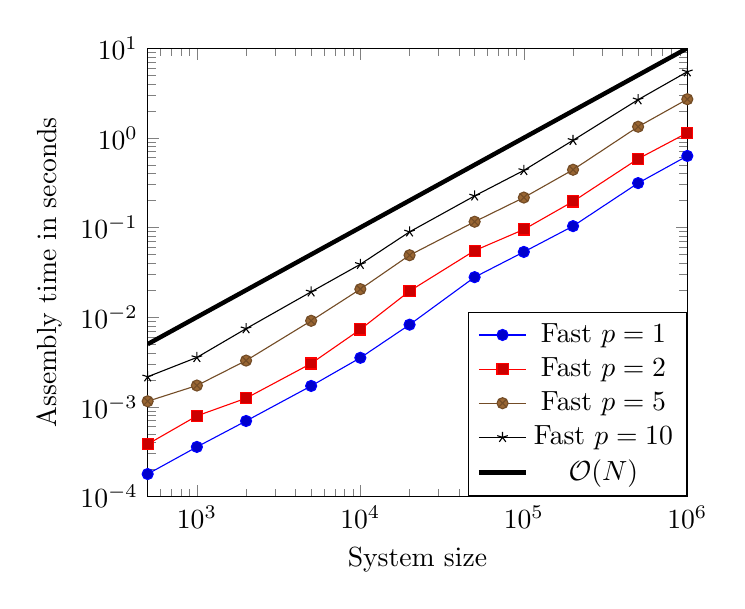
\begin{tikzpicture}
\begin{loglogaxis}[
	xlabel={System size},
	ylabel={Assembly time in seconds},
	xmin=500, xmax=1000000,
	ymin=1e-4, ymax=1e1,
	legend style={
  		at={(1.0,0.0)},
		anchor=south east},
]
%Fast p=1
\addplot
coordinates{
(500, 0.000178) (1000, 0.000357) (2000, 0.000695) (5000, 0.001709) (10000, 0.00352) (20000, 0.008242) (50000, 0.027928) (100000, 0.053394) (200000, 0.103547) (500000, 0.312632) (1000000, 0.628225) 
};
\addlegendentry{Fast $p=1$}
%Fast p=2
\addplot
coordinates{
(500, 0.000383) (1000, 0.000792) (2000, 0.001247) (5000, 0.003041) (10000, 0.007299) (20000, 0.019538) (50000, 0.055239) (100000, 0.095016) (200000, 0.195057) (500000, 0.583141) (1000000, 1.1374) 
};
\addlegendentry{Fast $p=2$}
%Fast p=5
\addplot
coordinates{
(500, 0.001153) (1000, 0.001728) (2000, 0.003278) (5000, 0.009105) (10000, 0.020535) (20000, 0.049057) (50000, 0.115912) (100000, 0.215703) (200000, 0.440508) (500000, 1.33005) (1000000, 2.69542) 
};
\addlegendentry{Fast $p=5$}
%Fast p=10
\addplot
coordinates{
(500, 0.002163) (1000, 0.003554) (2000, 0.007441) (5000, 0.019156) (10000, 0.038868) (20000, 0.089403) (50000, 0.224987) (100000, 0.433082) (200000, 0.938248) (500000, 2.66217) (1000000, 5.46193) 
};
\addlegendentry{Fast $p=10$}
%O(N) scaling
\addplot[ultra thick, no marks]
coordinates{
(500, 0.005) (1000000, 10)
};
\addlegendentry{$\mathcal{O}(N)$}
% %O(N^2) scaling
% \addplot
% coordinates{
% (500, 0.1) (5000, 10)
% };
% \addlegendentry{$\mathcal{O}(N^2)$}
% %Usual p=1
% \addplot
% coordinates{
% (500, 0.005261) (1000, 0.017753) (2000, 0.075765) (5000, 0.466064) (10000, 2.02409)
% };
% \addlegendentry{Usual $p=1$}
% %Usual p=2
% \addplot
% coordinates{
% (500, 0.00716) (1000, 0.027731) (2000, 0.100045) (5000, 0.614003) (10000, 2.57907)
% };
% \addlegendentry{Usual $p=2$}
% %Usual p=5
% \addplot
% coordinates{
% (500, 0.015521) (1000, 0.049203) (2000, 0.187864) (5000, 1.15643) (10000, 4.76131)
% };
% \addlegendentry{Usual $p=5$}
% %Usual p=10
% \addplot
% coordinates{
% (500, 0.023198) (1000, 0.084467) (2000, 0.327282) (5000, 2.04739) (10000, 8.36465)
% };
% \addlegendentry{Usual $p=10$}
\end{loglogaxis}
\end{tikzpicture}
\end{document}